% ==========================================================================
% European Journal of Physics (IOP Publishing) version of qsol_cqed.tex,
% using IOP's current iopjournal.cls template (2024).  On Overleaf: create the
% project from the "IOP Publishing" journal template (it ships iopjournal.cls and
% the orcid icon), replace main.tex with this file, and upload the figures into
% a folder named figures/.  Content is identical to the REVTeX version.
% Generated by scratchpad/make_ejp_iopjournal.py from paper/qsol_cqed.tex.
% Options: \documentclass[anonymous]{iopjournal} strips author details,
% acknowledgments and the data statement for double-anonymous review.
% ==========================================================================
\documentclass{iopjournal}
% graphicx, fancyhdr, xcolor and hyperref are loaded by the class.
\usepackage{amsmath}
\usepackage{amssymb}
\graphicspath{{figures/}{../figures/}}
% running head placeholders (volume/year/article number are set by the journal)
\fancyhead[L]{{\small \sf IOP Publishing}\hspace{5mm} {\it Eur. J. Phys.} {\bf vv} (yyyy) aaaaaa}
\fancyhead[R]{N K Nguyen}

\begin{document}

\articletype{Paper}

\title{Quantum states of light in cavity QED: a computational study of Wigner function dynamics and atom--field entanglement in the Jaynes--Cummings model}

% To add an ORCID iD use \orcid{0000-0000-0000-0000} after the name; it needs the
% "orcid" icon file that ships with the Overleaf IOP template.
\author{Nguyen Khoi Nguyen$^{1,2,*}$}

\affil{$^1$Department of Electrical and Computer Engineering, Boston University, Boston, MA 02215, United States of America}

\affil{$^2$Physics Department, Boston University, Boston, MA 02215, United States of America}

\affil{$^*$Author to whom any correspondence should be addressed.}

\email{nknguyen@bu.edu}  % confirm the address to be published

\keywords{Jaynes--Cummings model, Wigner function, Schr\"{o}dinger cat state, entanglement entropy, decoherence, cavity QED, computational physics education, QuTiP}

\begin{abstract}
The Jaynes--Cummings (JC) model is the standard first encounter with quantized light--matter interaction, yet most courses stop at the collapse and revival of Rabi oscillations and leave three of its most instructive lessons untaught: what the cavity field looks like in phase space while the oscillations are collapsed, how the atom--field entanglement evolves through a collapse--revival cycle, and how quickly cavity loss erases the non-classical features. We present a self-contained computational treatment of these questions for advanced undergraduate and beginning graduate students, in which every figure is generated by a short QuTiP script that the reader can run and modify. Starting from the dipole Hamiltonian we derive the JC model, its dressed states, and the collapse and revival times $t_c = O(1/g)$ and $t_r = 2\pi\sqrt{\bar{n}}/g$, then solve the Lindblad master equation for an initially excited atom and a coherent field with $\bar{n} = 10$. Three results organize the discussion. (i) At half the revival time the field is a Schr\"{o}dinger cat state with Wigner negativity $\delta = 0.85$, purity 0.96 and fidelity 0.78 to a two-component cat, and the atom has disentangled from it (reduced entropy $S \approx 0.14$~bit); during the preceding collapse the atom and field are instead maximally entangled and the reduced field is a two-branch mixture. (ii) Among coherent, thermal, squeezed and Fock initial fields, this half-revival disentanglement occurs only for the coherent field, and a thermal field saturates the reduced entropy at one bit while its logarithmic negativity stays near 0.2, showing why the reduced entropy measures entanglement only for pure global states. (iii) A cavity decay rate of $\kappa/g = 0.02$ removes over 80\% of the Wigner negativity. We close with exercises built on the code and a mapping of the results onto microwave and circuit-QED parameters.
\end{abstract}

\section{Introduction}
\label{sec:intro}

Coherent manipulation of quantum two-level systems is a cornerstone of quantum technology. Rabi oscillations, the periodic cycling of population between two quantum states under a resonant driving field, provide the physical mechanism for controlling qubit states~\cite{rabi1937, scully1997}. When a two-level system is driven on resonance, its state oscillates between the ground and excited state at a rate known as the Rabi frequency, which is set by the coupling strength to the field~\cite{allen1975, gerry2004}. By choosing the duration and phase of the driving pulse, one can prepare arbitrary superpositions or implement reliable state flips, operations essential for quantum gates.

The Jaynes--Cummings (JC) model~\cite{jaynes1963}, which describes the interaction of a single two-level atom with a single quantized cavity mode, is the simplest fully quantum model of light--matter interaction. Despite its simplicity, the JC model predicts a rich set of phenomena with no classical analog: vacuum Rabi splitting, collapse and revival of Rabi oscillations~\cite{eberly1980}, and the dynamical generation of Schr\"{o}dinger cat states in the cavity field~\cite{brune1996}. These predictions have been confirmed in pioneering cavity quantum electrodynamics (QED) experiments with Rydberg atoms in microwave cavities~\cite{rempe1987, haroche2006} and, more recently, in circuit QED with superconducting qubits coupled to microwave resonators~\cite{blais2021}.

While the JC model appears in every quantum-optics course, most presentations stop at the collapse and revival of the atomic inversion and leave three of its most instructive lessons untaught: what the cavity field looks like in phase space while the oscillations are collapsed, how the atom--field entanglement evolves through a collapse--revival cycle, and how quickly cavity loss erases the non-classical features. The lessons are not new to the research literature. Eberly \textit{et al.}~\cite{eberly1980} explained the collapse and revival, Gea-Banacloche~\cite{gea-banacloche1990, gea-banacloche1991} showed that the atom and field disentangle at half the revival time and leave the field in a Schr\"{o}dinger cat state, and Phoenix and Knight~\cite{phoenix1988, phoenix1991} traced the entanglement entropy through the cycle. They are, however, easy to misread. The cat state and the peak of the entanglement both occur while the inversion is collapsed, and it is tempting to identify one with the other; separating them requires watching the Wigner function, the field purity and the atomic entropy at the same time, which is exactly what a computational treatment makes cheap.

This paper is written for advanced undergraduate and beginning graduate students, and for instructors of quantum-optics or computational-physics courses. It assumes second quantization of a single mode, density matrices and the partial trace, and a first exposure to master equations; Section~\ref{sec:theory} supplies a self-contained derivation of the rest, and readers who know the JC model can proceed directly to Section~\ref{sec:methods}. Every figure is produced by a short, documented QuTiP~\cite{johansson2012, johansson2013} script that runs in seconds to a minute on a laptop, and the scripts are the intended instrument: the reader is meant to change $\bar{n}$, $\kappa/g$ or the initial field state and watch the figures respond. Section~\ref{sec:teaching} collects exercises built on that premise.

Our contribution relative to textbook treatments~\cite{gerry2004, haroche2006} is threefold. We compute the time-resolved Wigner function of the cavity field and quantify its non-classicality by the negativity volume; we compare the entanglement dynamics across coherent, thermal, squeezed-vacuum and Fock initial fields, using the reduced entropy where the global state is pure and the logarithmic negativity where it is mixed, so that the limits of the entropy as an entanglement measure become visible; and we quantify how cavity dissipation destroys the cat state. The pedagogical core is a three-regime picture: an entangled two-branch mixture during the collapse, a disentangled and nearly pure cat state at half the revival time, and re-entanglement at the revival.

The paper is organized as follows. Section~\ref{sec:theory} reviews the quantum states of light, the Wigner function, the JC Hamiltonian and its dressed states, and the collapse and revival timescales. Section~\ref{sec:methods} describes the computational methods, including the convergence checks that a student should reproduce. Section~\ref{sec:results} presents the simulation results. Section~\ref{sec:criteria} summarizes the criteria that distinguish classical from quantum light. Section~\ref{sec:experiment} maps the dimensionless results onto the platforms on which the phenomena have been observed. Section~\ref{sec:teaching} suggests how the material and the code can be used in a course, and Section~\ref{sec:conclusions} concludes.


\section{Theoretical Framework}
\label{sec:theory}

\subsection{Quantum harmonic oscillator and field quantization}
\label{sec:quantization}

Each mode of the electromagnetic field is a quantum harmonic oscillator. Writing the mode Hamiltonian as $H = \hbar\omega(a^\dagger a + \tfrac{1}{2})$ with $[a, a^\dagger] = 1$, the number operator $\hat{n} = a^\dagger a$ has the Fock states $|n\rangle$ as eigenstates, with $a^\dagger|n\rangle = \sqrt{n+1}\,|n+1\rangle$ and $a|n\rangle = \sqrt{n}\,|n-1\rangle$, and the single-mode electric field operator is $\hat{E}(t) = i\mathcal{E}_0\,(a e^{-i\omega t} - a^\dagger e^{i\omega t})$, where $\mathcal{E}_0 = \sqrt{\hbar\omega/(2\varepsilon_0 V)}$ is the field amplitude of one photon in the quantization volume $V$. The ground state carries the zero-point energy $\tfrac{1}{2}\hbar\omega$. The factor $\sqrt{n+1}$ in the action of $a^\dagger$ is the origin of every $\sqrt{n+1}$ that appears below, and the reader may wish to keep it in mind. Standard derivations are given in Refs.~\cite{scully1997, gerry2004}.


\subsection{Quantum states of light}
\label{sec:states}

\textit{Fock states} $|n\rangle$ are eigenstates of the photon number operator with a definite number of photons. They have no classical analog: a classical field cannot have an exact integer photon count. Fock states exhibit the quantum granularity of the field; for example, a single-photon state $|1\rangle$ produces at most one detection event, and the vacuum $|0\rangle$ produces none.

\textit{Coherent states} $|\alpha\rangle$, for complex amplitude $\alpha$, are the most important states in quantum optics. They are defined as eigenstates of the annihilation operator, $a|\alpha\rangle = \alpha|\alpha\rangle$, or equivalently as displaced vacuum states $|\alpha\rangle = D(\alpha)|0\rangle$ with displacement operator $D(\alpha) = \exp(\alpha a^\dagger - \alpha^* a)$. Expanding in the Fock basis yields a Poissonian photon-number distribution:
\begin{equation}
P_n = |\langle n|\alpha\rangle|^2 = e^{-|\alpha|^2} \frac{|\alpha|^{2n}}{n!},
\label{eq:poisson}
\end{equation}
with mean $\bar{n} = |\alpha|^2$ and variance $\text{Var}(n) = \bar{n}$. The equality of variance and mean is a hallmark of classical (shot-noise-limited) light. Coherent states minimize the Heisenberg uncertainty relation for field quadratures, with equal noise in both conjugate components at the vacuum level. They are often called the ``most classical'' quantum states because their mean electric field follows a classical sinusoid and their Glauber--Sudarshan $P$-distribution is a delta function, $P(\beta) = \delta^2(\beta - \alpha)$~\cite{glauber1963}. Laser light above threshold is well described by a coherent state with large $\bar{n}$.

\textit{Squeezed states} are non-classical states in which the quantum noise in one field quadrature is reduced below the vacuum level, at the expense of increased noise in the conjugate quadrature. Defining the quadrature $X_\phi = \tfrac{1}{2}(a e^{-i\phi} + a^\dagger e^{i\phi})$, a vacuum or coherent state has $\langle(\Delta X_\phi)^2\rangle = \tfrac{1}{4}$ independent of $\phi$ (in units with $\hbar = 1$). A squeezed state has $\langle(\Delta X_{\phi_0})^2\rangle < \tfrac{1}{4}$ for some optimal phase $\phi_0$. The squeeze operator $S(\zeta) = \exp[\tfrac{1}{2}(\zeta^* a^2 - \zeta a^{\dagger 2})]$ with $\zeta = r e^{i\varphi}$ applied to the vacuum yields uncertainties
\begin{equation}
\langle (\Delta X_{\varphi/2})^2 \rangle = \tfrac{1}{4} e^{-2r}, \quad
\langle (\Delta X_{\varphi/2 + \pi/2})^2 \rangle = \tfrac{1}{4} e^{2r}.
\label{eq:squeeze}
\end{equation}
Squeezed states can be produced by parametric down-conversion or four-wave mixing. Because they exhibit noise below the vacuum level in one observable, they have no classical description (their $P$-representation involves derivatives of delta functions). Since 2019, squeezed light has been injected into the LIGO and Virgo gravitational-wave observatories to reduce quantum noise, significantly improving sensitivity~\cite{aasi2013, tse2019}, a direct application of non-classical light to precision measurement.


\subsection{Phase-space representations: the Wigner function}
\label{sec:wigner}

The Wigner function provides a quasi-probability distribution in phase space that is particularly useful for visualizing quantum states and identifying non-classical features. For a single-mode field with density operator $\rho$, it is defined as~\cite{wigner1932}
\begin{equation}
W(x, p) = \frac{1}{\pi\hbar} \int_{-\infty}^{\infty} \langle x - y | \rho | x + y \rangle \, e^{2ipy/\hbar} \, dy,
\label{eq:wigner_def}
\end{equation}
where $x$ and $p$ are conjugate phase-space quadratures. Unlike a true probability distribution, $W(x,p)$ can take negative values; such negative regions are a sufficient (though not necessary) indicator of non-classicality~\cite{hudson1974}.

For a coherent state $|\alpha\rangle$, the Wigner function is a Gaussian centered at $(\sqrt{2}\,\text{Re}\,\alpha,\, \sqrt{2}\,\text{Im}\,\alpha)$:
\begin{equation}
W_\alpha(x,p) = \frac{1}{\pi} \exp\!\Big[-\big(x - \sqrt{2}\,\text{Re}\,\alpha\big)^2 - \big(p - \sqrt{2}\,\text{Im}\,\alpha\big)^2\Big],
\label{eq:wigner_coherent}
\end{equation}
which is everywhere non-negative. For a Fock state $|n\rangle$,
\begin{equation}
W_n(x,p) = \frac{(-1)^n}{\pi} \, L_n\!\big(2(x^2 + p^2)\big) \, e^{-(x^2 + p^2)},
\label{eq:wigner_fock}
\end{equation}
where $L_n$ is the $n$-th Laguerre polynomial; for $n \geq 1$ this exhibits pronounced negative regions. A squeezed vacuum has an elliptical Gaussian Wigner function with widths $e^{-r}$ and $e^{r}$ along the squeezed and anti-squeezed quadratures; it remains non-negative, though its $P$-representation is singular.

A quantitative measure of non-classicality is the Wigner negativity volume~\cite{kenfack2004}:
\begin{equation}
\delta = \int \big|W(x,p)\big| \, dx\, dp - 1.
\label{eq:negativity}
\end{equation}
Since $\int W\,dx\,dp = 1$, $\delta$ equals twice the integrated volume of the negative part of $W$. Every state with a non-negative Wigner function has $\delta = 0$; this includes all classical states but also, for example, the squeezed vacuum, so $\delta > 0$ is a sufficient but not a necessary witness of non-classicality. We use $\delta$ as a quantitative probe throughout the simulations in Sec.~\ref{sec:results}.


\subsection{Derivation of the Jaynes--Cummings Hamiltonian}
\label{sec:jcm}

We derive the Jaynes--Cummings model~\cite{jaynes1963} from the electric-dipole form of the light--matter interaction, the dipole-gauge counterpart of the minimal-coupling Hamiltonian $(\boldsymbol{p} - q\boldsymbol{A})^2/2m$ to which it is related by the Power--Zienau--Woolley transformation~\cite{scully1997}. In the dipole approximation, the interaction between a two-level atom and a single quantized cavity mode of frequency $\omega_c$ is
\begin{equation}
H_{\text{int}} = -\boldsymbol{d} \cdot \boldsymbol{E}(t),
\end{equation}
where $\boldsymbol{d}$ is the atomic dipole operator and $\boldsymbol{E}(t) \propto \boldsymbol{\varepsilon}(a + a^\dagger)$ is the quantized electric field, with $\boldsymbol{\varepsilon}$ the polarization vector. Restricting to two atomic levels $|g\rangle$ and $|e\rangle$ with transition frequency $\omega_a$, the dipole operator is $\boldsymbol{d} = \boldsymbol{d}_0(\sigma^+ + \sigma^-)$, where $\sigma^+ = |e\rangle\langle g|$, $\sigma^- = |g\rangle\langle e|$, and $\boldsymbol{d}_0$ is the transition dipole matrix element. The total Hamiltonian is then
\begin{equation}
H = \hbar\omega_c\, a^\dagger a + \frac{\hbar\omega_a}{2}\sigma_z + \hbar g(\sigma^+ + \sigma^-)(a + a^\dagger),
\label{eq:rabi_full}
\end{equation}
where $\sigma_z = |e\rangle\langle e| - |g\rangle\langle g|$ and the coupling constant $g$ is proportional to $\boldsymbol{d}_0 \cdot \boldsymbol{\varepsilon}$ and the single-photon field amplitude. Equation~(\ref{eq:rabi_full}) is the quantum Rabi model. It contains both energy-conserving terms ($a\sigma^+$ and $a^\dagger\sigma^-$) and counter-rotating terms ($a^\dagger\sigma^+$ and $a\sigma^-$) that do not conserve excitation number.

In the regime $g \ll \omega_a, \omega_c$ and near resonance ($|\omega_a - \omega_c| \ll \omega_a + \omega_c$), the counter-rotating terms oscillate at frequency $\omega_a + \omega_c$ in the interaction picture and average to zero. Dropping them gives the rotating-wave approximation (RWA) and the Jaynes--Cummings Hamiltonian:
\begin{equation}
H_{\text{JC}} = \hbar\omega_c\, a^\dagger a + \frac{\hbar\omega_a}{2}\sigma_z + \hbar g\left(a^\dagger \sigma^- + a\,\sigma^+\right).
\label{eq:HJC}
\end{equation}
The term $a^\dagger\sigma^-$ describes atomic de-excitation with photon emission, and $a\sigma^+$ describes photon absorption with atomic excitation. A key symmetry of $H_{\text{JC}}$ is conservation of the total excitation number $N = a^\dagger a + \sigma^+\sigma^-$, which commutes with $H_{\text{JC}}$. The Hilbert space therefore decomposes into invariant two-dimensional subspaces $\{|e, n\rangle,\, |g, n{+}1\rangle\}$ for each $n \in \mathbb{N}$, enabling exact analytic solutions.


\subsection{Dressed states and energy eigenvalues}
\label{sec:dressed}

Within the subspace of $n{+}1$ total excitations, the Hamiltonian in the basis $\{|e, n\rangle,\, |g, n{+}1\rangle\}$ reduces (after subtracting the common energy $(n + \tfrac{1}{2})\hbar\omega_c$) to the $2 \times 2$ matrix
\begin{equation}
H^{(n)} = \frac{\hbar}{2}
\begin{pmatrix}
\Delta & \Omega_0\sqrt{n+1} \\
\Omega_0\sqrt{n+1} & -\Delta
\end{pmatrix},
\label{eq:2x2}
\end{equation}
where $\Delta = \omega_a - \omega_c$ is the detuning and $\Omega_0 = 2g$ is the single-photon Rabi frequency. The coupling matrix element $\langle e, n | H_{\text{JC}} | g, n{+}1\rangle = \hbar g\sqrt{n+1}$ follows from the bosonic commutation relations. The eigenvalues are
\begin{equation}
E_{\pm}(n) = \hbar\omega_c\left(n + \tfrac{1}{2}\right) \pm \frac{\hbar}{2}\,\Omega_n(\Delta),
\label{eq:eigenvalues}
\end{equation}
where the generalized $n$-photon Rabi frequency is
\begin{equation}
\Omega_n(\Delta) = \sqrt{\Delta^2 + \Omega_0^2(n+1)}.
\label{eq:gen_rabi}
\end{equation}
The corresponding eigenstates (dressed states) are
\begin{align}
|n,+\rangle &= \cos\tfrac{\theta_n}{2}\, |e,n\rangle + \sin\tfrac{\theta_n}{2}\, |g,n{+}1\rangle, \label{eq:dressed_plus}\\
|n,-\rangle &= \sin\tfrac{\theta_n}{2}\, |e,n\rangle - \cos\tfrac{\theta_n}{2}\, |g,n{+}1\rangle, \label{eq:dressed_minus}
\end{align}
with mixing angle defined by $\tan\theta_n = \Omega_0\sqrt{n+1}/\Delta$. These are entangled atom--photon states whose character interpolates between atom-like and photon-like as $\Delta$ is varied. The energy splitting between the two dressed states is $\hbar\Omega_n(\Delta)$.


\subsection{Limiting cases}
\label{sec:limits}

\textit{Resonance} ($\Delta = 0$). The mixing angle is $\theta_n = \pi/2$ and the dressed states become equal superpositions:
\begin{equation}
|n, \pm\rangle = \frac{1}{\sqrt{2}}\left(|e,n\rangle \pm |g,n{+}1\rangle\right).
\end{equation}
The splitting reduces to $\hbar\Omega_0\sqrt{n+1}$. For $n = 0$ (one total excitation), the splitting is $\hbar\Omega_0 = 2\hbar g$, the vacuum Rabi splitting. This is directly analogous to the normal-mode splitting of two coupled oscillators, and its spectroscopic observation~\cite{thompson1992} was among the first confirmations of the JC model.

\textit{Large detuning} ($|\Delta| \gg \Omega_0\sqrt{n+1}$). The mixing angle is small and the dressed states are only weakly entangled. Expanding $\Omega_n \approx |\Delta| + \Omega_0^2(n+1)/(2|\Delta|)$ gives energy shifts
\begin{equation}
E_\pm(n) \approx \hbar\omega_c\left(n + \tfrac{1}{2}\right) \pm \frac{\hbar}{2}\left(|\Delta| + \frac{\Omega_0^2(n+1)}{2|\Delta|}\right).
\end{equation}
The second-order corrections $\propto g^2/\Delta$ are the ac Stark (light) shifts~\cite{haroche2006}. In this regime the eigenstates approach the bare states $|e,n\rangle$ and $|g,n{+}1\rangle$, and the atom--field coupling manifests primarily as dispersive frequency shifts rather than coherent population transfer. The transition from resonant Rabi splitting to dispersive shifts as $\Delta$ is varied produces an avoided crossing of width $\hbar\Omega_0\sqrt{n+1}$ at $\Delta = 0$.


\subsection{Rabi oscillations from a Fock-state field}
\label{sec:rabi_fock}

Consider the atom initially excited and the field in a Fock state with $n$ photons: $|\Psi(0)\rangle = |e, n\rangle$. This state is not an eigenstate of the coupled system; it is a superposition of the two dressed states in the $(n{+}1)$-excitation manifold. On resonance,
\begin{equation}
|e, n\rangle = \frac{1}{\sqrt{2}}\left(|n,+\rangle + |n,-\rangle\right).
\end{equation}
Evolving each eigenstate with its eigenphase gives the time-dependent state (dropping the common phase):
\begin{equation}
|\Psi(t)\rangle = \cos\!\left(\tfrac{1}{2}\Omega_n t\right)|e,n\rangle - i\sin\!\left(\tfrac{1}{2}\Omega_n t\right)|g,n{+}1\rangle,
\label{eq:rabi_evolution}
\end{equation}
where $\Omega_n = \Omega_0\sqrt{n+1}$ and the sign of the second term follows from $e^{-iH_{\text{JC}}t/\hbar}$ with the coupling $+\hbar g(a^\dagger\sigma^- + a\sigma^+)$. The excited-state probability oscillates sinusoidally:
\begin{equation}
P_e(t) = \cos^2\!\left(\frac{\Omega_0\sqrt{n+1}}{2}\,t\right),
\label{eq:pe_fock}
\end{equation}
at the $n$-photon Rabi frequency $\Omega_n = \Omega_0\sqrt{n+1}$. For $n = 0$, this is the vacuum Rabi oscillation: an excited atom in an empty cavity emits and reabsorbs a single photon periodically at frequency $\Omega_0$. For $n \gg 1$, the Rabi frequency $\Omega_0\sqrt{n+1} \approx \Omega_0\sqrt{n}$ is proportional to the classical field amplitude $\propto \sqrt{n}$, recovering the semiclassical limit. These coherent oscillations require the strong-coupling regime ($g \gg \kappa, \gamma$) so that the photon is not lost from the cavity during a Rabi cycle~\cite{haroche2006}.


\subsection{Collapse and revival of Rabi oscillations}
\label{sec:collapse_revival}

Now suppose the atom is initially excited and the field is in a coherent state $|\alpha\rangle$ with mean photon number $\bar{n} = |\alpha|^2$. Expanding the coherent state in the Fock basis,
\begin{equation}
|\Psi(0)\rangle = |e\rangle \otimes |\alpha\rangle = e^{-\bar{n}/2}\sum_{n=0}^{\infty} \frac{\alpha^n}{\sqrt{n!}}\,|e, n\rangle,
\end{equation}
and evolving each Fock component independently via Eq.~(\ref{eq:rabi_evolution}), the excited-state probability at time $t$ is
\begin{equation}
P_e(t) = \sum_{n=0}^{\infty} p(n)\,\cos^2\!\left(\frac{\Omega_0\sqrt{n+1}}{2}\,t\right),
\label{eq:pe_coherent}
\end{equation}
where $p(n) = e^{-\bar{n}}\bar{n}^n/n!$ is the Poisson distribution. Using the identity $\cos^2\theta = \tfrac{1}{2}(1 + \cos 2\theta)$,
\begin{equation}
P_e(t) = \frac{1}{2} + \frac{1}{2}\sum_{n=0}^{\infty} p(n)\,\cos\!\left(\Omega_0\sqrt{n+1}\,t\right).
\label{eq:pe_cos_sum}
\end{equation}
Equation~(\ref{eq:pe_cos_sum}) is a weighted superposition of cosines at incommensurate frequencies $\Omega_0\sqrt{n+1}$. The Poisson weights are peaked around $n \approx \bar{n}$ with width $\sqrt{\bar{n}}$, so at short times all components oscillate nearly in phase at the dominant frequency $\Omega_0\sqrt{\bar{n}+1}$.

\textit{Collapse.} As time progresses, the components dephase because neighboring Fock states oscillate at slightly different frequencies. The spread of Rabi frequencies across the Poisson distribution (width $\sigma_n = \sqrt{\bar{n}}$) is
\begin{equation}
\delta\Omega \sim \frac{\partial\Omega_n}{\partial n}\bigg|_{\bar{n}} \cdot \sigma_n = \frac{\Omega_0}{2\sqrt{\bar{n}}} \cdot \sqrt{\bar{n}} = \frac{\Omega_0}{2}.
\end{equation}
The oscillations dephase when $\delta\Omega \cdot t_c \sim 1$, giving the collapse time
\begin{equation}
t_c \sim \frac{2}{\Omega_0} = \frac{1}{g},
\label{eq:t_collapse}
\end{equation}
independent of $\bar{n}$~\cite{eberly1980}. The numerical prefactor depends on the criterion adopted: linearizing $\sqrt{n+1}$ about $\bar{n}$ and summing Eq.~(\ref{eq:pe_cos_sum}) over the approximately Gaussian Poisson weights gives the envelope $P_e(t) - \tfrac{1}{2} \approx \tfrac{1}{2}\cos(\Omega_0\sqrt{\bar{n}}\,t)\,e^{-g^2t^2/2}$, whose $1/e$ time is $\sqrt{2}/g$. Throughout this paper we use the operational definition $t_c \equiv 1/g$; in the simulations the oscillations are fully damped by $t \approx 2t_c$. After the collapse, $P_e(t)$ fluctuates around $1/2$ with negligible amplitude.

\textit{Revival.} Despite the apparent loss of coherence, the oscillations return at a later time. Because the Rabi frequencies are $\Omega_0\sqrt{n+1}$ (a discrete set, not a continuum), the phases can realign modulo $2\pi$. To estimate the revival time, we require adjacent Fock components near $n \approx \bar{n}$ to accumulate a phase difference of exactly $2\pi$:
\begin{equation}
\left(\Omega_0\sqrt{n+2} - \Omega_0\sqrt{n+1}\right) t_r = 2\pi.
\end{equation}
For large $n$, $\sqrt{n+2} - \sqrt{n+1} \approx 1/(2\sqrt{n+1})$, giving
\begin{equation}
t_r \approx \frac{4\pi\sqrt{\bar{n}}}{\Omega_0} = \frac{2\pi\sqrt{\bar{n}}}{g}.
\label{eq:t_revival}
\end{equation}
The ratio $t_r/t_c \approx 2\pi\sqrt{\bar{n}}$ shows that for large $\bar{n}$, the revival occurs many collapse times later, with a broad plateau of near-zero oscillation amplitude in between.

The revival is a purely quantum effect. A classical field with a continuous amplitude distribution would produce irreversible dephasing with no recurrence. The revival requires the \textit{discrete} spectrum of Fock-state Rabi frequencies, and its observation constitutes direct evidence that the intracavity field is quantized~\cite{eberly1980, haroche2006}.

After the first revival, the components dephase again on a timescale $\sim t_c$, producing a second collapse. Further revivals occur quasi-periodically at integer multiples of $t_r$, though higher-order revivals become progressively less sharp as the accumulated phase errors grow~\cite{gerry2004}.

For a thermal field (photon statistics given by the Bose--Einstein distribution, $p(n) = \bar{n}^n/(1+\bar{n})^{n+1}$), the distribution is much broader than Poisson ($\sigma_n \sim \bar{n}$ rather than $\sqrt{\bar{n}}$). The dephasing is correspondingly faster, and no pronounced revival is resolved within the simulated window; the evolution nevertheless remains unitary, so this is a loss of visibility rather than a strictly irreversible process. This contrast between coherent and thermal fields is a central result of our simulations (Sec.~\ref{sec:entropy_results}).

During the collapse the atom and field become strongly entangled. Remarkably, at half the revival time, $t_r/2 = \pi\sqrt{\bar{n}}/g$, the two branches of the atomic state reconverge onto a common state that is independent of the initial atomic state, so that the atom and field approximately \emph{disentangle}, and the field is left in a nearly pure Schr\"{o}dinger cat state, a superposition of two coherent states with opposite phases~\cite{gea-banacloche1990, gea-banacloche1991, phoenix1991}. This connection between Rabi collapse, transient entanglement, half-revival disentanglement, and cat-state formation is a central theme of our computational results.


\subsection{Open quantum systems: the Lindblad master equation}
\label{sec:lindblad}

Real cavity QED systems are coupled to their environment. The dominant dissipation channels are cavity photon loss at rate $\kappa$ and atomic spontaneous emission into non-cavity modes at rate $\gamma$. Within the Markov approximation, the density matrix evolves according to the Lindblad master equation~\cite{lindblad1976, wiseman2009}:
\begin{equation}
\frac{d\rho}{dt} = -\frac{i}{\hbar}[H_{\text{JC}}, \rho] + \kappa\, \mathcal{D}[a]\rho + \gamma\, \mathcal{D}[\sigma^-]\rho,
\label{eq:lindblad}
\end{equation}
where the Lindblad dissipator is
\begin{equation}
\mathcal{D}[L]\rho = L\rho L^\dagger - \frac{1}{2}\big(L^\dagger L \rho + \rho L^\dagger L\big).
\label{eq:dissipator}
\end{equation}
The strong-coupling regime, where quantum coherent effects dominate, requires $g \gg \kappa, \gamma$ so that the atom and field exchange energy many times before dissipation destroys coherence. In this regime, vacuum Rabi splitting is spectroscopically resolvable and collapse-revival dynamics can unfold before being damped.

Dissipation has a particularly dramatic effect on the cat states generated during JC dynamics. The decoherence rate of the interference fringes of a superposition of two coherent states separated by $\Delta\alpha$ in phase space is $\kappa|\Delta\alpha|^2/2$~\cite{zurek2003, haroche2006}; for the JC cat, whose components sit at $\pm i\sqrt{\bar{n}}$ (Sec.~\ref{sec:wigner_results}), this is $2\kappa\bar{n}$, far exceeding the bare cavity decay rate $\kappa$. This rapid fragility of mesoscopic superpositions is a central result of our simulations.


\subsection{Atom--field entanglement: von Neumann entropy}
\label{sec:entropy_theory}

For a bipartite pure state $|\Psi\rangle_{AF}$ of the atom--field system, the degree of entanglement is uniquely quantified by the von Neumann entropy of either reduced subsystem~\cite{nielsen2000}:
\begin{equation}
S(\rho_{\text{atom}}) = -\text{Tr}\big[\rho_{\text{atom}} \log_2 \rho_{\text{atom}}\big],
\label{eq:entropy}
\end{equation}
where $\rho_{\text{atom}} = \text{Tr}_{\text{field}}(|\Psi\rangle\langle\Psi|)$. For a two-level atom, $S$ ranges from 0 (product state) to 1~bit (maximally entangled). The entropy is related to the purity of the reduced field state,
\begin{equation}
\mathcal{P} = \text{Tr}\big[\rho_{\text{field}}^2\big],
\label{eq:purity}
\end{equation}
which equals unity for product states and decreases with increasing entanglement.

Equation~(\ref{eq:entropy}) is an entanglement measure only when the global atom--field state is pure. If the global state is mixed, as for a thermal initial field or whenever dissipation acts, $S(\rho_{\text{atom}})$ counts classical as well as quantum correlations and can saturate at 1~bit for a weakly entangled state. In those cases we use the logarithmic negativity~\cite{vidal2002, plenio2005}
\begin{equation}
E_{\mathcal{N}} = \log_2 \big\| \rho^{T_{\text{atom}}} \big\|_1,
\label{eq:logneg}
\end{equation}
where $T_{\text{atom}}$ denotes partial transposition with respect to the atom and $\|\cdot\|_1$ the trace norm. $E_{\mathcal{N}}$ is an entanglement monotone for mixed states; it vanishes for separable states and equals 1 for a maximally entangled atom--field pair.

In the JC model, the entanglement dynamics are directly correlated with the collapse and revival of Rabi oscillations~\cite{phoenix1988}. As the oscillations collapse, the atom becomes strongly entangled with the field ($S \to 1$~bit). At half the revival time, however, the system approximately refactorizes: $S$ passes through a minimum, the atom approaches a pure state, and the field is left in a nearly pure cat state~\cite{gea-banacloche1990, phoenix1991}. Around the full revival the branches rephase and the entanglement grows again. This entropy--inversion correspondence was first analyzed by Phoenix and Knight~\cite{phoenix1988, phoenix1991}, and we verify it computationally in Sec.~\ref{sec:results}.


\section{Computational Methods}
\label{sec:methods}

All simulations are performed using QuTiP (Quantum Toolbox in Python, version~5.2)~\cite{johansson2012, johansson2013}, an open-source framework for simulating open and closed quantum systems. The cavity field is represented in a truncated Fock basis $\{|0\rangle, |1\rangle, \ldots, |N_{\text{cav}}-1\rangle\}$, and the joint atom--field Hilbert space has dimension $2N_{\text{cav}}$.

\textit{Fock space truncation.} The truncation is chosen per initial state. For the coherent and Fock states with $\bar{n} = 10$ we use $N_{\text{cav}} = 35$--$50$: the Poisson weight beyond $n = 35$ is below $10^{-9}$, and every quantity reported at $t_r/2$ (entropy, purity, $\delta$) agrees to four digits between $N_{\text{cav}} = 35$, 50, and 70. Thermal and squeezed-vacuum fields have much heavier photon-number tails (geometric, and $\propto \tanh^{2m}r/\sqrt{m}$ for $n = 2m$, respectively): at $N_{\text{cav}} = 50$ the truncated states would have $\langle n\rangle = 9.57$ and $9.15$ instead of 10, so for these we use $N_{\text{cav}} = 150$, which reproduces $\langle n\rangle = 10$ to four digits and leaves a truncated weight below $10^{-6}$. For the $\bar{n}$ scan we use $N_{\text{cav}} = 3\bar{n} + 20$. Trace normalization alone is not used as a convergence criterion.

\textit{Time evolution.} All propagation uses QuTiP's \texttt{mesolve} (version 5.2.3) with its default adaptive-step Adams--Moulton multistep integrator (\texttt{method='adams'}, absolute and relative tolerances $10^{-8}$ and $10^{-6}$). Pure initial states without dissipation are propagated as state vectors; the thermal initial field and all dissipative runs [Eq.~(\ref{eq:lindblad})] propagate the full density matrix.

\textit{Wigner functions.} At each snapshot time, we obtain the reduced field state $\rho_{\text{field}}(t) = \text{Tr}_{\text{atom}}[\rho(t)]$ via partial trace, then compute $W(x,p)$ on a $200 \times 200$ grid over $[-7, 7]^2$ (spacing 0.07, i.e.\ ten points per interference fringe of spacing $\pi/\sqrt{2\bar{n}} \approx 0.70$) using QuTiP's \texttt{wigner} function~\cite{johansson2012} in the convention $a = (x + ip)/\sqrt{2}$, for which $\int W\,dx\,dp = 1$ (verified to $10^{-4}$ on the grid). The negativity $\delta$ of Eq.~(\ref{eq:negativity}) is evaluated on the same grid.

\textit{Entanglement and cat-state measures.} The von Neumann entropy $S(\rho_{\text{atom}})$ is computed at each time step from the eigenvalues of the $2 \times 2$ reduced atomic density matrix, the field purity $\mathcal{P}(t) = \text{Tr}[\rho_{\text{field}}^2]$ directly, and the logarithmic negativity of Eq.~(\ref{eq:logneg}) from the trace norm of the partially transposed joint state. The cat-state fidelity is $F_{\text{cat}} = \max\,\langle \text{cat}|\rho_{\text{field}}|\text{cat}\rangle$ over normalized states $|\text{cat}\rangle \propto |\beta\rangle + e^{i\theta}|{-\beta}\rangle$, with $\beta$ scanned in a neighborhood of $i\sqrt{\bar{n}}$ and $\theta \in [0, 2\pi)$.

\textit{Parameters.} We work in dimensionless units with $g = 1$. The characteristic timescales are the collapse time $t_c \equiv 1/g$ and the revival time $t_r = 2\pi\sqrt{\bar{n}}/g$. Table~\ref{tab:params} summarizes the simulation parameters.

\begin{table}
\centering
\caption{Simulation parameters. All quantities in units where $g = 1$ and $\hbar = 1$.}
\begin{tabular}{lcccc}
\hline
Simulation & $\bar{n}$ & $N_{\text{cav}}$ & $\kappa/g$ & $\gamma/g$ \\
\hline
Wigner evolution & 10 & 35 & 0 & 0 \\
Entanglement (coherent, Fock) & 10 & 50 & 0 & 0 \\
Entanglement (thermal, squeezed) & 10 & 150 & 0 & 0 \\
$\bar{n}$ scaling & 1--36 & $3\bar{n}+20$ & 0 & 0 \\
Dissipative dynamics & 10 & 35--50 & 0--0.2 & 0 \\
\hline
\end{tabular}
\label{tab:params}
\end{table}

All simulation code is available as Python scripts at \url{https://github.com/alanknguyen/QSOL_CQED}.


\section{Results and Discussion}
\label{sec:results}

\subsection{Wigner function evolution and cat-state formation}
\label{sec:wigner_results}

We first consider unitary JC dynamics with the atom initially excited and the field in a coherent state $|\alpha\rangle$ with $\bar{n} = |\alpha|^2 = 10$. Figure~\ref{fig:inversion_snapshots} shows the atomic inversion $\langle\sigma_z(t)\rangle$, exhibiting the collapse-revival structure: rapid Rabi oscillations that dephase by $t \approx 2/g$, a quiescent interval, and a revival centered at $t_r \approx 2\pi\sqrt{10}/g \approx 19.9/g$.

\begin{figure}
\centering
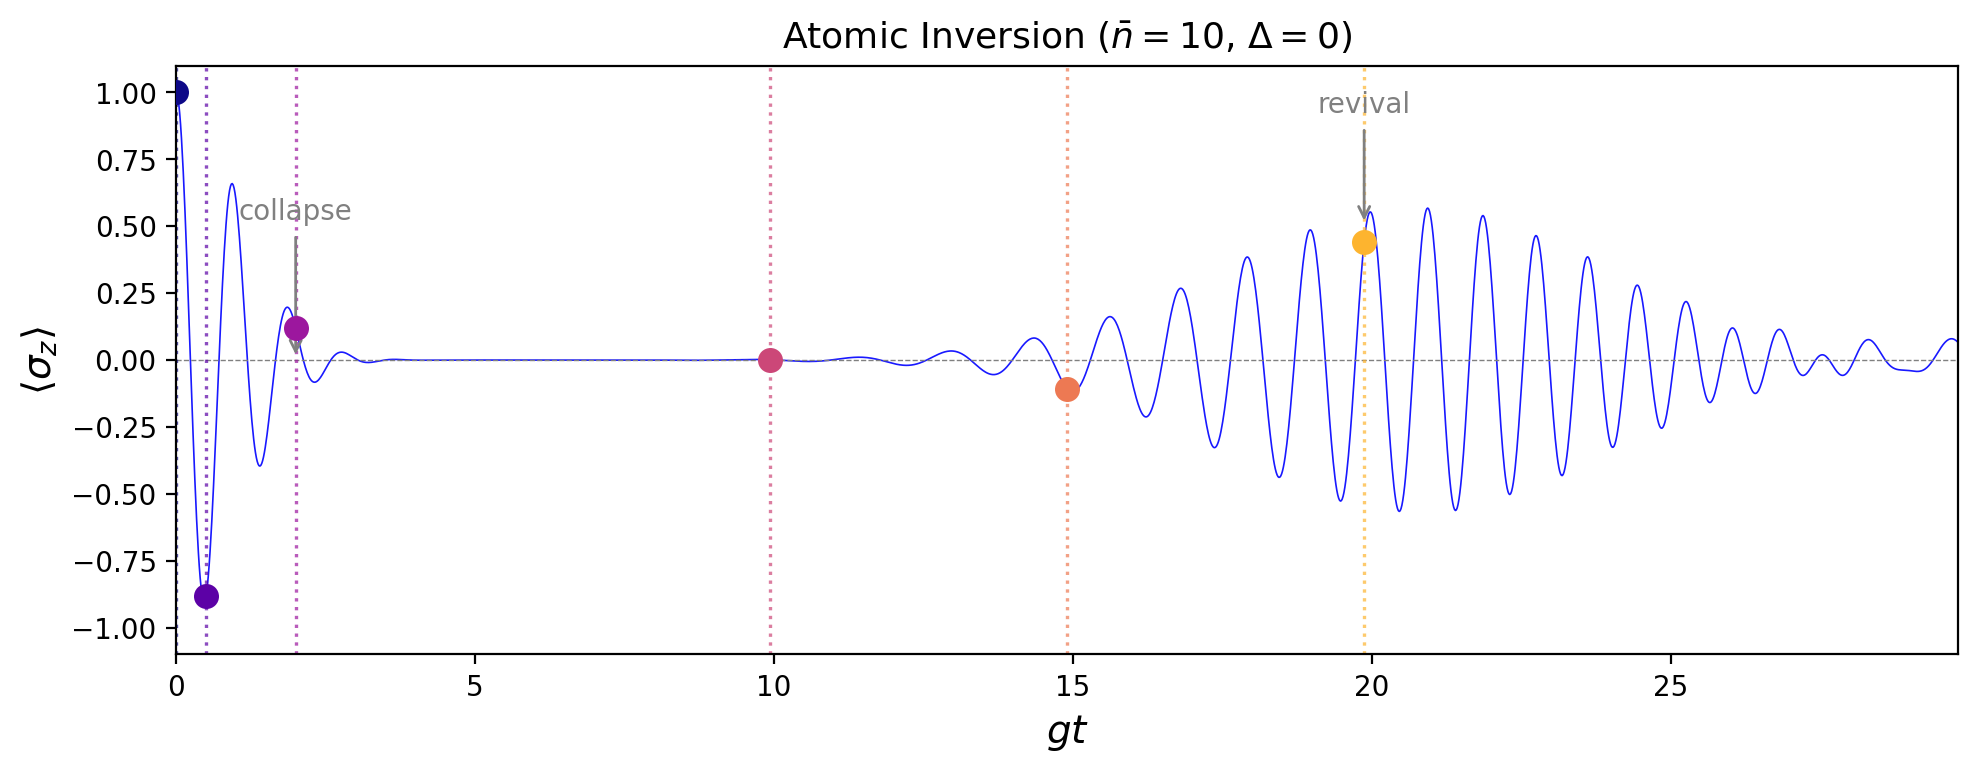
\includegraphics[width=\textwidth]{fig_inversion_snapshots.png}
\caption{Atomic inversion $\langle\sigma_z(t)\rangle$ for a two-level atom interacting with a coherent-state field ($\bar{n} = 10$) in the resonant Jaynes--Cummings model. Colored markers indicate the six snapshot times used for the Wigner function evolution in Fig.~\ref{fig:wigner_evolution}. The collapse of oscillations near $t \approx 2/g$ and the first revival at $t_r \approx 19.9/g$ are clearly visible.}
\label{fig:inversion_snapshots}
\end{figure}

\begin{figure}
\centering

\includegraphics[width=\textwidth]{fig_wigner_evolution.png}
\caption{Wigner function $W(x,p)$ of the reduced cavity field state at six characteristic times during Jaynes--Cummings evolution ($\bar{n} = 10$, $\Delta = 0$). At $t = 0$, the field is a coherent-state Gaussian. By $t = 2\,t_c$ (collapse onset), the distribution begins to spread. At $t = t_r/2$, a Schr\"{o}dinger cat state has formed: two distinct lobes at $p \approx \pm\sqrt{2\bar{n}}$ connected by interference fringes with strong Wigner negativity ($\delta = 0.85$); at this time the atom and field are approximately disentangled (Sec.~\ref{sec:entropy_results}). By $t = t_r$, the field partially re-localizes at revival ($\delta = 0.31$).}
\label{fig:wigner_evolution}
\end{figure}

The central computational result of this section is shown in Fig.~\ref{fig:wigner_evolution}, which displays the Wigner function of the reduced cavity field at six characteristic times. At $t = 0$, the Wigner function is a Gaussian displaced to $x \approx 4.5$, consistent with the initial coherent state. As the system evolves through the collapse region ($t \approx 2/g$), the distribution spreads along the circle $x^2 + p^2 = 2\bar{n}$ in phase space. At the midpoint of the collapse--revival cycle ($t = t_r/2$), the Wigner function develops two well-separated lobes connected by interference fringes with alternating positive and negative values, the signature of a Schr\"{o}dinger cat state, $|\Psi_{\text{cat}}\rangle \approx \mathcal{N}(|\beta\rangle + e^{i\theta}|{-\beta}\rangle)$ with $\beta \approx i\sqrt{\bar{n}}$: the two components sit on the $p$ axis, rotated by $\pm\pi/2$ from the initial coherent amplitude.

Figure~\ref{fig:cat_detail} provides a detailed view of this cat state. The cross-section $W(x, p = 0)$ shows deep negative excursions reaching $W \approx -0.25$, with Wigner negativity volume $\delta = 0.85$ (compared to $\delta = 0$ at $t = 0$). The best-fitting two-component cat has fidelity $F_{\text{cat}} = 0.78$ with the reduced field state, whose purity is $\mathcal{P} = 0.96$: the field is a nearly pure cat state rather than one branch of an entangled atom--field pair (Sec.~\ref{sec:entropy_results}). The relative phase of the fit is $\theta \approx 1.2\pi$ and the photon-number parity is $\langle(-1)^{\hat{n}}\rangle = -0.64$, so the JC cat is closer to an odd than to an even cat, and its photon-number distribution displays the corresponding odd-$n$ comb; its fidelity with the even cat $|\alpha\rangle + |{-\alpha}\rangle$ on the real axis is essentially zero. The interference fringes have characteristic spacing $\Delta x \approx \pi/\sqrt{2\bar{n}} \approx 0.7$, set by the separation of the two coherent components. These fringes are the phase-space manifestation of quantum interference between macroscopically distinguishable field states and serve as a definitive marker of non-classicality.

\begin{figure}
\centering

\includegraphics[width=\textwidth]{fig_cat_state_detail.png}
\caption{Detailed view of the Schr\"{o}dinger cat state formed at $t = t_r/2$. Left: Wigner function contour plot showing two coherent-state lobes and interference fringes. Right: cross-section $W(x, p=0)$ with negative regions (shaded red) reaching $W \approx -0.25$; the fringe spacing is $\pi/\sqrt{2\bar{n}} \approx 0.70$. The negativity ($\delta = 0.85$) confirms the non-classical character of this dynamically generated state, whose fidelity with the best-fitting two-component cat is 0.78.}
\label{fig:cat_detail}
\end{figure}

As the system approaches the revival time, the two lobes merge and the Wigner function partially re-localizes, though with residual non-classical features ($\delta = 0.31$ at $t = t_r$). The revival is not exact: higher-order terms in the photon-number distribution prevent perfect recurrence.


\subsection{Atom--field entanglement dynamics}
\label{sec:entropy_results}

We now quantify atom--field entanglement, comparing four initial field states with the same mean photon number $\bar{n} = 10$: coherent, thermal, squeezed vacuum, and Fock. For the three pure initial fields the global state remains pure and $S(\rho_{\text{atom}})$ is the entanglement entropy; for the thermal field we report both $S$ and the logarithmic negativity $E_{\mathcal{N}}$ of Eq.~(\ref{eq:logneg}).

Figure~\ref{fig:entanglement_comparison} shows the inversion, entropy, and negativity for all four cases. The principal observations are as follows.

\begin{figure}
\centering

\includegraphics[width=0.85\textwidth]{fig_entanglement_comparison.png}
\caption{Comparison of Jaynes--Cummings dynamics for four initial field states with $\bar{n} = 10$. (a) Atomic inversion $\langle\sigma_z\rangle$ for the coherent (blue), thermal (red), and squeezed-vacuum (green) fields. (b) Fock state $|10\rangle$ over a short window: the inversion oscillates with period $\pi/(g\sqrt{11})$ and the entropy (plotted as $2S - 1$) with half that period. (c) Reduced-atom entropy $S(\rho_{\text{atom}})$ (solid) and logarithmic negativity $E_{\mathcal{N}}$ (dashed). The coherent state collapses to $S \approx 1$~bit and disentangles at $t_r/2$ (dotted line); the thermal state saturates at $S = 1$~bit but has $E_{\mathcal{N}} \approx 0.2$ because its global state is mixed; the squeezed vacuum shows only partial dips. The dashed purple line marks the revival time $t_r$.}
\label{fig:entanglement_comparison}
\end{figure}

\textit{Coherent state.} The entropy rises from $S = 0$ to $\approx 1$~bit within $t \approx 2/g$, as the Rabi oscillations collapse. It then decreases steadily and reaches a minimum $S \approx 0.14$~bit ($E_{\mathcal{N}} = 0.36$) at $t = t_r/2 \approx 9.9/g$, in the middle of the quiescent interval. This is the half-revival disentanglement predicted by Gea-Banacloche~\cite{gea-banacloche1990}: the atom returns close to a pure state while the field is in the cat state of Fig.~\ref{fig:cat_detail}. Toward the revival the entanglement grows again; at $t_r$ the entropy is $S \approx 0.79$~bit and oscillates between about 0.5 and 1 at the Rabi frequency. The cat state and the minimum of entanglement therefore coincide: the field is a nearly pure superposition, not one branch of an entangled pair.

\textit{Thermal state.} The reduced entropy rises to $S = 1$~bit within $t \sim 1/g$ and stays within a few percent of the maximum thereafter, with no dip at $t_r/2$. This does not indicate maximal entanglement: the global state is mixed, and the logarithmic negativity remains small, $E_{\mathcal{N}} \approx 0.23$ on average (maximum 0.33). Most of the reduced-atom entropy is classical correlation inherited from the broad Bose--Einstein photon distribution, whose spread of Rabi frequencies ($\sigma_n \sim \bar{n}$) dephases the oscillations within a Rabi period and leaves no resolved revival in the simulated window.

\textit{Squeezed vacuum.} The dynamics are intermediate: a rapid rise to $S \approx 1$~bit followed by quasi-periodic partial dips (to $S \approx 0.7$--$0.8$), but no clean half-revival disentanglement. The super-Poissonian photon statistics of the squeezed vacuum (only even $n$ populated, variance $2\bar{n}(\bar{n}+1)$) spread the Rabi frequencies over a much wider range than the Poisson distribution.

\textit{Fock state.} With a definite photon number there is a single Rabi frequency, $\Omega_{10} = 2g\sqrt{11}$ [Eq.~(\ref{eq:rabi_evolution})]. The inversion oscillates with period $\pi/(g\sqrt{11}) \approx 0.95/g$, and the entropy, which depends on the populations only through the binary entropy $h(P_e)$ with $h(p) = h(1-p)$, oscillates between 0 and 1~bit with half that period, $\pi/(2g\sqrt{11}) \approx 0.47/g$ [Fig.~\ref{fig:entanglement_comparison}(b)]. No collapse or revival occurs because there is no dephasing.

Figure~\ref{fig:coherent_detail} shows the coherent-state case in greater detail, plotting inversion, entropy, and field purity $\mathcal{P}(t)$ together. During the collapse the field purity drops to $\mathcal{P} \approx 0.5$: the reduced field is then an incoherent \emph{mixture} of two nearly orthogonal branches, each correlated with a different atomic state (a coherent superposition of the two branches would have $\mathcal{P} = 1$). As the atomic branches reconverge, the purity climbs to $\mathcal{P} = 0.96$ at $t_r/2$, where the field is the nearly pure cat, and falls again toward the revival ($\mathcal{P} = 0.64$ at $t_r$). The three observables thus tell a single story: entanglement during the collapse turns the reduced field into a two-branch mixture, and disentanglement at $t_r/2$ restores the field's coherence in the form of a cat state.

\begin{figure}
\centering

\includegraphics[width=0.85\textwidth]{fig_coherent_entropy_purity.png}
\caption{Detailed coherent-state dynamics ($\bar{n} = 10$). Top: atomic inversion. Middle: entanglement entropy $S(\rho_{\text{atom}})$, peaking near 1~bit during the collapse and reaching its minimum ($\approx 0.14$~bit) at $t_r/2$, where the atom and field disentangle and the field is the cat state of Fig.~\ref{fig:cat_detail}. Bottom: field purity $\mathcal{P} = \text{Tr}[\rho_{\text{field}}^2]$, dropping to $\approx 0.5$ during the collapse (a two-branch mixture, the field being entangled with the atom) and rising to 0.96 at $t_r/2$ (nearly pure cat). Dotted and dashed lines mark $t_r/2$ and $t_r$.}
\label{fig:coherent_detail}
\end{figure}

Figure~\ref{fig:entropy_nbar} shows how these dynamics depend on $\bar{n}$. For $\bar{n} = 1$ the entropy oscillates quasi-periodically without a clean collapse. As $\bar{n}$ increases, the collapse still occurs at $t \sim 1/g$, but the half-revival minimum at $\pi\sqrt{\bar{n}}/g$ moves out and deepens ($S_{\min} \approx 0.16$, 0.11, 0.07, and 0.05~bit for $\bar{n} = 9$, 16, 25, and 36), and the entangled plateau around the revival broadens. For $\bar{n} \gtrsim 9$ the disentanglement and the subsequent re-entanglement are cleanly resolved, consistent with the large-$\bar{n}$ analysis of Gea-Banacloche~\cite{gea-banacloche1991}.

\begin{figure}
\centering

\includegraphics[width=\textwidth]{fig_entropy_nbar_scaling.png}
\caption{Entanglement entropy $S(\rho_{\text{atom}})$ for coherent-state fields with $\bar{n} = 1,\, 4,\, 9,\, 16,\, 25,\, 36$. As $\bar{n}$ increases, the collapse time remains $\sim 1/g$ while the half-revival time $\pi\sqrt{\bar{n}}/g$ (dotted) and the revival time $t_r = 2\pi\sqrt{\bar{n}}/g$ (dashed) grow as $\sqrt{\bar{n}}$. The entropy minimum at $t_r/2$ (atom--field disentanglement) deepens with $\bar{n}$ and is cleanly resolved for $\bar{n} \gtrsim 9$.}
\label{fig:entropy_nbar}
\end{figure}


\subsection{Decoherence of non-classical features}
\label{sec:decoherence}

We now include cavity photon loss ($\kappa > 0$) via Eq.~(\ref{eq:lindblad}) and study its effect on the Wigner function and entanglement.

Figure~\ref{fig:wigner_decoherence} shows the Wigner function at the cat-state time $t = t_r/2$ for $\kappa/g = 0,\, 0.02,\, 0.05,\, 0.10$. The interference fringes are progressively destroyed: at $\kappa/g = 0.02$, the Wigner negativity drops from $\delta = 0.85$ to $\delta = 0.14$; at $\kappa/g = 0.10$, the negativity is effectively zero ($\delta = 0.002$). Table~\ref{tab:decoherence} summarizes these results; the values are converged to three digits between $N_{\text{cav}} = 35$ and 50.

\begin{figure}
\centering

\includegraphics[width=\textwidth]{fig_wigner_decoherence.png}
\caption{Decoherence of the Schr\"{o}dinger cat state. Wigner function at $t = t_r/2$ for increasing cavity decay rates $\kappa/g = 0,\, 0.02,\, 0.05,\, 0.10$ (left to right). The interference fringes are progressively destroyed; quantitative values of the Wigner negativity $\delta$ are given in Table~\ref{tab:decoherence}.}
\label{fig:wigner_decoherence}
\end{figure}

\begin{table}
\centering
\caption{Wigner negativity $\delta$ and field purity $\mathcal{P}$ at $t = t_r/2$ for varying cavity decay rate, with $\bar{n} = 10$.}
\begin{tabular}{cccc}
\hline
$\kappa/g$ & Wigner negativity $\delta$ & Field purity $\mathcal{P}$ & Cat state visible? \\
\hline
0.00 & 0.851 & 0.960 & Yes \\
0.02 & 0.143 & 0.460 & Marginal \\
0.05 & 0.022 & 0.418 & No \\
0.10 & 0.002 & 0.386 & No \\
\hline
\end{tabular}
\label{tab:decoherence}
\end{table}

This extreme sensitivity is expected: the fringe decoherence rate is $2\kappa\bar{n}$ (Sec.~\ref{sec:lindblad}). For $\bar{n} = 10$, even $\kappa/g = 0.02$ gives a fringe-decoherence time $1/(2\kappa\bar{n}) = 2.5/g$, a quarter of the cat-formation time $t_r/2 \approx 10/g$, which suffices to wash out most of the interference while the two Gaussian lobes, which decay only at the rate $\kappa$, persist.

Figure~\ref{fig:dissipative_entropy} shows the inversion, the reduced entropy, and the logarithmic negativity under dissipation. Three effects are visible. (i) The Rabi revival is damped and the inversion relaxes toward $\langle\sigma_z\rangle \to -1$ as photons leak out; for $\kappa/g = 0.2$ the atom is essentially in its ground state by $gt \approx 30$. (ii) The reduced entropy no longer measures entanglement: for $\kappa/g \geq 0.05$ it saturates near 1~bit at late times while the negativity decays toward zero ($E_{\mathcal{N}} = 0.14$, 0.02, and 0.00 at $gt = 30$ for $\kappa/g = 0.05$, 0.10, and 0.20). (iii) The atom--field entanglement at $t_r/2$ is comparatively robust: $E_{\mathcal{N}}(t_r/2) \approx 0.35$ for all $\kappa/g \leq 0.1$, close to the unitary value 0.36, even though the entropy minimum is progressively filled in [$S(t_r/2) = 0.14$, 0.16, 0.27, and 0.49 for $\kappa/g = 0$, 0.01, 0.05, and 0.10] and the cat fringes of Table~\ref{tab:decoherence} are already gone at $\kappa/g = 0.05$. Cavity loss thus destroys the internal coherence of the field cat long before it changes the (small) residual entanglement between atom and field.

\begin{figure}
\centering

\includegraphics[width=0.85\textwidth]{fig_dissipative_entanglement.png}
\caption{Effect of cavity decay on JC dynamics ($\bar{n} = 10$). Top: atomic inversion for $\kappa/g = 0$--$0.20$. Middle: reduced-atom entropy, which for $\kappa > 0$ measures total (classical plus quantum) correlations. Bottom: logarithmic negativity $E_{\mathcal{N}}$, a proper entanglement monotone for the mixed states produced by dissipation. Increasing $\kappa$ damps the revival, drives the atom toward its ground state, and suppresses the late-time negativity even where the reduced entropy stays near 1~bit. Dotted and dashed lines mark $t_r/2$ and $t_r$.}
\label{fig:dissipative_entropy}
\end{figure}

These results demonstrate the challenge of maintaining quantum coherence. By the operational criterion $\delta > 0.05$ at $t_r/2$, cat-state formation with $\bar{n} = 10$ requires $\kappa/g \lesssim 0.03$, i.e.\ $g/\kappa \gtrsim 30$; the threshold depends on $\bar{n}$, on the observation time, and on the chosen figure of merit (a full map of $\delta$ and $F_{\text{cat}}$ over the $(\bar{n}, \kappa/g)$ plane is provided with the code). This condition is routinely achieved in microwave cavity QED~\cite{haroche2006} and circuit QED~\cite{blais2021}, but remains an engineering challenge in optical cavities.


\section{Classical vs.\ Quantum Light: Criteria for Quantum Engineering}
\label{sec:criteria}

The computational results above illustrate the distinction between classical and quantum light in a dynamical setting. Here we summarize the formal criteria and their relevance to quantum technologies.

The Glauber--Sudarshan $P$-distribution~\cite{glauber1963, sudarshan1963} provides the gold-standard test. If a state's density matrix can be written as $\rho = \int P(\alpha) |\alpha\rangle\langle\alpha|\,d^2\alpha$ with a non-negative, well-behaved $P(\alpha)$, the state is classical (a mixture of coherent states). States for which $P(\alpha)$ is more singular than a delta function or takes negative values, including Fock states and squeezed states, are non-classical. The Wigner function being negative is a sufficient but not necessary indicator; the Husimi $Q$-function is always positive and thus less sensitive.

Photon statistics provide experimentally accessible tests. Sub-Poissonian statistics (Mandel $Q < 0$) or photon antibunching ($g^{(2)}(0) < 1$) cannot occur with classical fields. The observation of $g^{(2)}(0) \approx 0$ in single-atom fluorescence~\cite{kimble1977} was the first definitive proof of quantum light. Conversely, photon bunching ($g^{(2)}(0) = 2$) is expected for thermal light and does not imply non-classicality.

Squeezing below the vacuum level is another definitive quantum signature. No classical state can have less noise in any quadrature than the vacuum. The injection of squeezed vacuum into the Advanced LIGO detectors has reduced the quantum shot noise by up to $\approx 3$~dB at frequencies above $\sim 50$~Hz, which was estimated to raise the detection rate for binary-neutron-star mergers by 40--50\%~\cite{tse2019}.

These criteria matter because non-classical light enables quantum technologies that surpass classical limits: squeezed states improve interferometric sensitivity beyond the standard quantum limit; entangled photon pairs enable quantum key distribution~\cite{ekert1991}; and NOON states can achieve Heisenberg-limited phase sensitivity scaling as $1/N$ rather than the shot-noise $1/\sqrt{N}$.


\section{Connection to Experiment}
\label{sec:experiment}

The collapse-revival phenomenon remained a theoretical prediction for over two decades after the original JC model~\cite{jaynes1963} and the analysis by Eberly \textit{et al.}~\cite{eberly1980}, because its observation requires a single two-level system coupled to a single quantized mode in the strong-coupling regime $g \gg \kappa, \gamma$. It has since been seen on four platforms. Rempe, Walther, and Klein~\cite{rempe1987} observed the first quantum revivals with Rydberg atoms crossing a superconducting microwave cavity one at a time; the same platform later yielded the generation and detection of cat states~\cite{brune1996} and quantum non-demolition counting of photons~\cite{haroche2006}, with $g/2\pi \sim 50$~kHz and $\kappa/2\pi \sim 1$~Hz. Meekhof \textit{et al.}~\cite{meekhof1996} reproduced the full collapse-revival sequence with a single trapped $^9$Be$^+$ ion whose vibrational mode plays the role of the cavity field, demonstrating that the physics belongs to any two-level system coupled to a quantized boson mode. In optical cavities, Thompson, Rempe, and Kimble~\cite{thompson1992} resolved the vacuum Rabi splitting of a single cesium atom, confirming the $n = 1$ dressed-state structure, although short optical cavity lifetimes make time-domain revivals difficult. In circuit QED~\cite{blais2021}, superconducting qubits coupled to microwave resonators with $g/2\pi \sim 100$--$300$~MHz and $\kappa/2\pi \sim 1$~MHz reach $g/\kappa \sim 100$--$300$; Hofheinz \textit{et al.}~\cite{hofheinz2009} verified the $\sqrt{n+1}$ scaling of the Rabi frequency with synthesized Fock states, and Ofek \textit{et al.}~\cite{ofek2016} used cat states in a superconducting cavity for quantum error correction beyond the break-even point.

Our dimensionless results map onto these platforms by inserting the physical value of $g$. For the microwave cavity QED parameters above ($g = 2\pi \times 50$~kHz) the revival time for $\bar{n} = 10$ is $t_r = 2\pi\sqrt{10}/g \approx 60~\mu$s, far shorter than the cavity lifetime $1/\kappa \approx 0.16$~s; for circuit QED it is $t_r \approx 10$--$30$~ns against $1/\kappa \approx 160$~ns. In both cases the first revival occurs well within the coherence time. The cat-state fringes, which decohere at the enhanced rate $2\kappa\bar{n}$, survive only where $\kappa/g \lesssim 0.01$--$0.03$, which is why the $g/\kappa \gtrsim 30$ threshold of Sec.~\ref{sec:decoherence} is met in the microwave and circuit-QED regimes but not in typical optical cavities.


\section{Using this material in teaching}
\label{sec:teaching}

This study grew out of a term project in a graduate course on quantum optics at Boston University (EC~585/777) and is organized so that it can be reused in that role.

\textit{Where it fits.} The natural place is immediately after the JC model and the collapse-revival phenomenon have been introduced, in a quantum-optics or cavity-QED course at advanced-undergraduate or first-year-graduate level, or as a case study in a computational-physics module. Prerequisites are second quantization of a single mode, density matrices and the partial trace, and a first exposure to the Lindblad equation; Section~\ref{sec:theory} supplies the rest. Three lectures cover the content: (a) collapse and revival as dephasing and rephasing of a discrete spectrum, using Figs.~\ref{fig:inversion_snapshots} and \ref{fig:entropy_nbar}; (b) the field in phase space, the cat state and its decoherence, using Figs.~\ref{fig:wigner_evolution}, \ref{fig:cat_detail} and \ref{fig:wigner_decoherence} and Table~\ref{tab:decoherence}; (c) entanglement measures and their limits, using Figs.~\ref{fig:entanglement_comparison}, \ref{fig:coherent_detail} and \ref{fig:dissipative_entropy}.

\textit{Misconceptions the figures are designed to confront.} Four statements are tempting and wrong, and each is refuted by a figure the student can regenerate. First, that the cat state forms when the atom and field are maximally entangled: Fig.~\ref{fig:coherent_detail} shows the entropy at its minimum, not its maximum, when the cat appears. Second, that a field purity of one half signals a superposition of two states: it signals a mixture, and the coherent superposition arrives only when the purity returns to 0.96 at $t_r/2$. Third, that a reduced entropy of one bit means maximal entanglement: for the thermal field of Fig.~\ref{fig:entanglement_comparison} the logarithmic negativity is only about 0.2, because the global state is mixed. Fourth, that a non-negative Wigner function implies a classical state: the squeezed vacuum has $\delta = 0$ and is nonetheless non-classical (Sec.~\ref{sec:criteria}).

\textit{Exercises.} All of the following run in seconds to a minute on a laptop with the scripts in the repository.
\begin{enumerate}
\item Change $\bar{n}$ in the Wigner-evolution script to 4, 16 and 25 and verify from the inversion that $t_r$ scales as $\sqrt{\bar{n}}$ while the collapse is complete by $t \approx 2/g$ regardless.
\item Derive the entropy period $\pi/(2g\sqrt{n+1})$ of the Fock state from Eq.~(\ref{eq:rabi_evolution}) and the symmetry $h(p) = h(1-p)$ of the binary entropy, then confirm it against panel (b) of Fig.~\ref{fig:entanglement_comparison}.
\item Reproduce Table~\ref{tab:decoherence} and extend it to $\kappa/g = 0.01$ and $0.03$; locate the decay rate at which $\delta$ falls below 0.05, and compare with the naive estimate obtained by equating the fringe-decoherence time $1/(2\kappa\bar{n})$ to the formation time $t_r/2$. Explain why the estimate is too conservative.
\item Using the closed form $P(n,t) = p(n)\cos^2(g\sqrt{n+1}\,t) + p(n-1)\sin^2(g\sqrt{n}\,t)$ for the photon-number distribution, show that $P(n, t_r/2)$ alternates with the parity of $n$, and compare the predicted parity $\langle(-1)^{\hat{n}}\rangle$ with the numerical value $-0.64$ quoted in Sec.~\ref{sec:wigner_results}.
\item Repeat the thermal-field simulation with $N_{\text{cav}} = 50$ instead of 150 and explain, from the initial $\langle n\rangle$, why the truncation must be chosen per initial state. This is the convergence check that separates a simulation from a picture.
\item (Advanced) Add a detuning $\Delta \neq 0$ to the Hamiltonian and investigate how the half-revival cat fidelity and the entropy minimum change; relate the result to the dispersive limit of Sec.~\ref{sec:limits}.
\end{enumerate}

\textit{Assessment.} A suitable project is to produce the three-observable portrait of Fig.~\ref{fig:coherent_detail} for a different initial state, for example a displaced Fock state or an initial atomic superposition, and to explain in one page where the cat forms, when the atom and field disentangle, and what the logarithmic negativity adds to the reduced entropy.


\section{Conclusions}
\label{sec:conclusions}

We have presented a computational treatment of the Jaynes--Cummings model intended for teaching, in which the collapse and revival of Rabi oscillations, the phase-space dynamics of the cavity field, and the atom--field entanglement are followed together from reproducible code. Three lessons emerge that standard presentations leave implicit. First, the Schr\"{o}dinger cat state that forms at half the revival time, with Wigner negativity $\delta = 0.85$, purity 0.96 and cat fidelity 0.78, coincides with a \emph{minimum} of the atom--field entanglement ($S \approx 0.14$~bit): it is a nearly pure state of the field alone, whereas during the preceding collapse the atom and field are maximally entangled and the reduced field is a two-branch mixture. Second, the half-revival disentanglement first analyzed by Gea-Banacloche~\cite{gea-banacloche1990} and by Phoenix and Knight~\cite{phoenix1988, phoenix1991} is unique to the coherent field, and for a thermal field a saturated reduced entropy of one bit conceals a logarithmic negativity of only about 0.2, so that once the global state is mixed the reduced entropy must not be read as an entanglement measure. Third, cavity decay as weak as $\kappa/g = 0.02$ removes over 80\% of the Wigner negativity while leaving the residual atom--field negativity at $t_r/2$ nearly unchanged, which separates the loss of the field's internal coherence from the loss of entanglement.

The physics is classical work; what the computational route adds is that the three observables can be placed side by side at negligible cost, and that each of the misconceptions listed in Sec.~\ref{sec:teaching} becomes a figure a student can regenerate and then break by changing a parameter. The scripts extend without modification to detuned, multi-mode and ultrastrong-coupling variants of the model, and to quantum-trajectory simulations of individual measurement records.


\ack{The author thanks Prof.\ Luca Dal Negro for guidance and feedback during the preparation of this work (EC 585 and EC 777, Boston University).}

% \funding{This work received no external funding.}
% \roles{N K N carried out all the work reported.}

\data{The simulation code that generates every figure in this article, together with the raw sweep data, is openly available at \url{https://github.com/alanknguyen/QSOL_CQED}. All results were obtained with QuTiP 5.2.3.}

% \suppdata{...}

% thebibliography prints the "References" heading itself in this (article-based) class
\begin{thebibliography}{99}
\bibitem{rabi1937} Rabi I I 1937 {\it Phys. Rev.} {\bf 51} 652
\bibitem{scully1997} Scully M O and Zubairy M S 1997 {\it Quantum Optics} (Cambridge: Cambridge University Press)
\bibitem{allen1975} Allen L and Eberly J H 1975 {\it Optical Resonance and Two-Level Atoms} (New York: Dover)
\bibitem{gerry2004} Gerry C C and Knight P L 2004 {\it Introductory Quantum Optics} (Cambridge: Cambridge University Press)
\bibitem{jaynes1963} Jaynes E T and Cummings F W 1963 {\it Proc. IEEE} {\bf 51} 89
\bibitem{eberly1980} Eberly J H, Narozhny N B and Sanchez-Mondragon J J 1980 {\it Phys. Rev. Lett.} {\bf 44} 1323
\bibitem{brune1996} Brune M, Hagley E, Dreyer J, Ma\^{\i}tre X, Maali A, Wunderlich C, Raimond J M and Haroche S 1996 {\it Phys. Rev. Lett.} {\bf 77} 4887
\bibitem{rempe1987} Rempe G, Walther H and Klein N 1987 {\it Phys. Rev. Lett.} {\bf 58} 353
\bibitem{haroche2006} Haroche S and Raimond J-M 2006 {\it Exploring the Quantum: Atoms, Cavities, and Photons} (Oxford: Oxford University Press)
\bibitem{blais2021} Blais A, Grimsmo A L, Girvin S M and Wallraff A 2021 {\it Rev. Mod. Phys.} {\bf 93} 025005
\bibitem{glauber1963} Glauber R J 1963 {\it Phys. Rev.} {\bf 131} 2766
\bibitem{sudarshan1963} Sudarshan E C G 1963 {\it Phys. Rev. Lett.} {\bf 10} 277
\bibitem{aasi2013} Aasi J {\it et al} (LIGO Scientific Collaboration) 2013 {\it Nat. Photon.} {\bf 7} 613
\bibitem{tse2019} Tse M {\it et al} (LIGO Scientific Collaboration) 2019 {\it Phys. Rev. Lett.} {\bf 123} 231107
\bibitem{wigner1932} Wigner E 1932 {\it Phys. Rev.} {\bf 40} 749
\bibitem{hudson1974} Hudson R L 1974 {\it Rep. Math. Phys.} {\bf 6} 249
\bibitem{kenfack2004} Kenfack A and \.{Z}yczkowski K 2004 {\it J. Opt. B: Quantum Semiclass. Opt.} {\bf 6} 396
\bibitem{thompson1992} Thompson R J, Rempe G and Kimble H J 1992 {\it Phys. Rev. Lett.} {\bf 68} 1132
\bibitem{lindblad1976} Lindblad G 1976 {\it Commun. Math. Phys.} {\bf 48} 119
\bibitem{wiseman2009} Wiseman H M and Milburn G J 2009 {\it Quantum Measurement and Control} (Cambridge: Cambridge University Press)
\bibitem{zurek2003} Zurek W H 2003 {\it Rev. Mod. Phys.} {\bf 75} 715
\bibitem{nielsen2000} Nielsen M A and Chuang I L 2000 {\it Quantum Computation and Quantum Information} (Cambridge: Cambridge University Press)
\bibitem{phoenix1988} Phoenix S J D and Knight P L 1988 {\it Ann. Phys. (N.Y.)} {\bf 186} 381
\bibitem{johansson2012} Johansson J R, Nation P D and Nori F 2012 {\it Comput. Phys. Commun.} {\bf 183} 1760
\bibitem{johansson2013} Johansson J R, Nation P D and Nori F 2013 {\it Comput. Phys. Commun.} {\bf 184} 1234
\bibitem{gea-banacloche1990} Gea-Banacloche J 1990 {\it Phys. Rev. Lett.} {\bf 65} 3385
\bibitem{gea-banacloche1991} Gea-Banacloche J 1991 {\it Phys. Rev.} A {\bf 44} 5913
\bibitem{phoenix1991} Phoenix S J D and Knight P L 1991 {\it Phys. Rev.} A {\bf 44} 6023
\bibitem{vidal2002} Vidal G and Werner R F 2002 {\it Phys. Rev.} A {\bf 65} 032314
\bibitem{plenio2005} Plenio M B 2005 {\it Phys. Rev. Lett.} {\bf 95} 090503
\bibitem{kimble1977} Kimble H J, Dagenais M and Mandel L 1977 {\it Phys. Rev. Lett.} {\bf 39} 691
\bibitem{ekert1991} Ekert A K 1991 {\it Phys. Rev. Lett.} {\bf 67} 661
\bibitem{hofheinz2009} Hofheinz M, Wang H, Ansmann M, Bialczak R C, Lucero E, Neeley M, O'Connell A D, Sank D, Wenner J, Martinis J M and Cleland A N 2009 {\it Nature} {\bf 459} 546
\bibitem{ofek2016} Ofek N {\it et al} 2016 {\it Nature} {\bf 536} 441
\bibitem{meekhof1996} Meekhof D M, Monroe C, King B E, Itano W M and Wineland D J 1996 {\it Phys. Rev. Lett.} {\bf 76} 1796
\end{thebibliography}

\end{document}
